\documentclass[12pt]{article}
\usepackage[a4paper, margin=.30in]{geometry}
\usepackage{graphicx ,
            wrapfig,
            xcolor, 
            enumerate,
            amsmath,fontenc, mhchem  ,tcolorbox 
            }

\newcommand\headerMe[2]{\noindent{}#1\hfill#2}
\renewcommand{\thesection}{\Roman{section}}

\author{Zakaria HAOUZAN}
\date{\today}

\begin{document}
% headers --------------
\headerMe{Matière : Physique-Chimie}{Professeur : Zakaria HAOUZAN}\\
\headerMe{Unité : Travail Mécanique et Energie }{Établissement : Lycée SKHOR qualifiant}\\
\headerMe{Niveau : 1BAC-SM-X}{Heure : 4H}\\

% ------Content ________
\begin{center}

    \Large{Leçon $N^{\circ} 6 $: \color{red}Dosages (ou titrages) directs }
\end{center}

%\begin{wrapfigure}[10]{r}{0.5\textwidth}
%    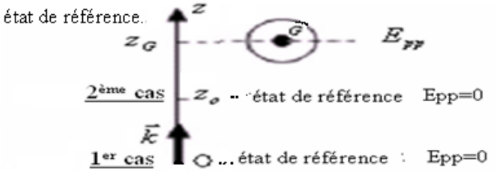
\includegraphics[width=0.5\textwidth]{./img/img00.png}
%\end{wrapfigure}


%\begin{tcolorbox}[colback=pink!10!white,
                  %colframe=blue!15!gray,
                  %title=Application -1- :
                 %]



\section{Principe d’un dosage : }
\subsection{Définition }
Le dosage (ou titrage) consiste à déterminer la concentration d'une espèce chimique présente dans une solution dite
solution titrée, en faisant réagir cette solution avec une solution de concentration connue dite solution titrante.
La réaction du dosage doit vérifier les conditions suivantes:
\\- Elle doit être rapide. (l'état final du système est atteint dans une courte durée).
\\-Elle doit totale (le réactif limitant est toujours entièrement consommé).
\\-Elle doit être unique (Elle ne doit pas être en compétition avec d'autres réactions)
\begin{wrapfigure}[10]{r}{0.3\textwidth}
  \vspace{-2cm}
    \includegraphics[width=0.3\textwidth]{./img/Mode_opératoire_dosage:.png}
\end{wrapfigure}
  \subsection{Mode opératoire d'un dosage:}
On introduit dans un bécher à l'aide d'une pissette jaugée un volume de la solution à titrer .Puis on lui ajoute
progressivement à l'aide d'une burette la solution titrante. On utilise un système d'agitation afin d'homogénéiser le
mélange.

  \subsection{L'équivalence:}
Au début et avant l'équivalence le réactif titrant est limitant.(car il disparait complètement dès qu'on l'introduit dans le
bécher).

  En continuant à ajouter le réactif titrant le réactif titré se consomme progressivement jusqu'à sa disparition complète:
( à ce moment l'équivalence est atteint , le mélange réactionnel devient stœchiométrique).

  Après l'équivalence le réactif titré est limitant (car il a disparaît complètement du milieu réactionnel) .
On peut repérer le point d'équivalence par l'une des méthodes suivantes:
\\-Soit par changement de la couleur du mélange réactionnel (cas des réactions d'oxydoréductions).
\\-Soit par changement de la couleur d'un indicateur coloré (cas de réactions acido-basiques).
\\-Soit en traçant la courbe de la variation d'une grandeur physique par suivi de son évolution en fonction du volume
versé de la solution titrante. (Cas du dosage conductimétrique ou dosage par pH-métrie)
  \begin{wrapfigure}[10]{r}{0.4\textwidth}
    \vspace{-0.6cm}
    \includegraphics[width=0.4\textwidth]{./img/Dosage conductimétrique.png}
\end{wrapfigure}
  
  \begin{wrapfigure}[10]{r}{0.5\textwidth}
\vspace{-1.8cm}
    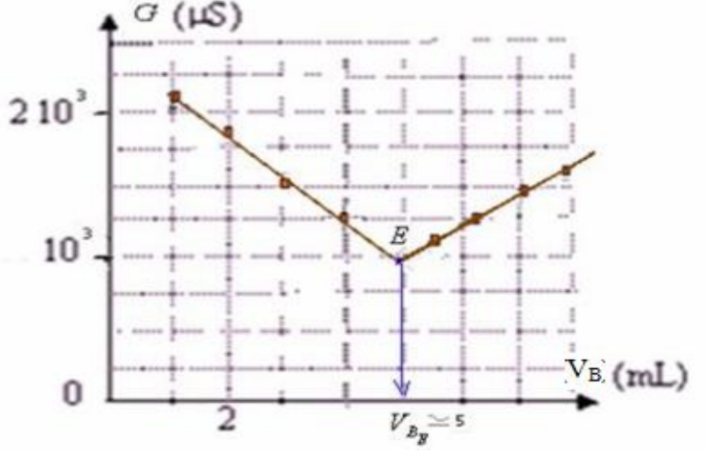
\includegraphics[width=0.5\textwidth]{./img/courbe dosage conduc.png}
\end{wrapfigure}
  \section{Réalisation d’un dosage direct}
  \subsection{Dosage conductimétrique:}
  \subsubsection{Mode opératoire:}
Pour réaliser le dosage d'une solution $S_1$ d'acide chlorhydrique ( $H_3O^+ + Cl^-$ ) par une solution $S_2$ d'hydroxyde de sodium
( $Na^+ + HO^-$ ) de concentration molaire $c_B=10^{-2} mol/L$ , on verse un volume $V_A=25mL$ de la solution $S_1$ dans un bécher et lui ajoute progressivement à l'aide d'une burette graduée la solution $S_2$ d'hydroxyde de sodium tout en mesurant la
variation de la conductance du mélange réactionnel en fonction de la variation du volume de soude ajouté.
On trace la courbe : G=f($V_B$)
  \subsubsection{Interprétation:}
  La courbe représentant G en fonction de VB présente deux parties rectilignes qui se coupent en un point E (point d'équivalence) qui correspond au volume $V_{BE}$ de soude versé à l'équivalence.

  Avant l'équivalence les ions oxonium $H_3O^+$qui se trouvent en excès dans le bécher et qui ont une grande conductivité molaire ionique se consomment progressivement au cour du dosage et ils sont remplacés par les ions $Na^+$ qui ont une faible conductivité molaire ionique :
\\ce qui explique la diminution de la conductance de la solution.

  Après l'équivalence, les ions oxonium $H_3O^+$ sont totalement consommés, les ions $HO^-$ ajoutés s'accumulent dans le mélange ce qui entraine la croissance de la conductance.
\subsubsection{Relation d'équivalence:}
Les ions $Na^+$ de la solution de soude et les ions $Cl^-$ de la solution d'acide chlorhydrique sont inactifs ( ils ne participent pas à la réaction ).

Donc l'équation de la réaction du dosage s'écrit :
$$\ce{$H_3O^+$ + $HO^-$ -> $2H_2O$}$$
Tableau d'avancement de la réaction:

% table dont forget 
\begin{center}
\begin{tabular}{|c|c|c|c|c|}
    \hline
    \multicolumn{2}{|c|}{Equation de la réaction}& \multicolumn{3}{c|}{ $H_3O^+$ + $HO^- \rightarrow 2H_2O$}\\\hline
    états  & avancement& \multicolumn{3}{|c|}{quantité de Matière en mol}\\\hline
    Etat initial          & 0 &$C_A.V_A$  &$C_B.V_{Bver}$ & excès  \\\hline
    Etat de transformation&$x$&$C_A.V_A-x$&$C_B.V_{Bver}-x$& excès  \\\hline
    Etat final            &    $x_{max}$& $ C_A.V_A-x_{max}$ & $ C_B.V_{Bver}-x_{max}$&excès   \\\hline
   % \cline{2-4}\
\end{tabular}
\end{center}
A l'équivalence $V_Bvers=V_B$éq et le mélange est stœchiométrique , c'est à dire que les deux réactifs sont limitant.

donc on a  $C_A.V_A - x_{max} = 0 $ et $C_B.V_B - x_{max} = 0 $ Relation d'équivalence : $C_A.V_A = C_B.V_Beq$ 
$$C_A = \frac{C_B.V_Beq}{V_A} = 0.02mol/L$$

\begin{tcolorbox}[colback=pink!10!white,
                  colframe=blue!15!gray,
                  title=Conclusion : 
                 ]
  la courbe  $\sigma= f(V_{titrant}$ ) présente 2 demi-droites de pentes différentes.
  - Le point d’intersection de ces 2 demi-droites est le point équivalent E ( $ V_E, \sigma{E}$).

Un titrage conductimétrique est utilisé dans le cas ou la concentration des espèces ioniques varient au cours du
dosage.

\end{tcolorbox}


\subsection{Dosage colorimétrique:}
\subsubsection{Mode opératoire:}
Pour titrer une solution de sulfate de fer II ( $Fe^{2+} + SO_4^{2-}$ ) par une solution de permanganate de potassium ( $K^+ + MnO_4^- $) ,on introduit dans un bécher un volume $V_1=20mL$ d'une solution de sulfate de fer II de concentration $C_1$ inconnue puis lui ajoute progressivement à l'aide d'une burette une solution de permanganate de potassium de concentration $C_2=3.10^{-2}mol/L$ et qui est acidifié par quelques gouttes d'acide sulfurique. 
\begin{center}
\includegraphics[width=0.5\textwidth]{./img/dosage colorimétrique.png}
\end{center}
On utilise un agitateur magnétique durant le dosage pour rendre le mélange homogène.

On continue à ajouter la une solution de permanganate de potassium jusqu'au point d'équivalence qui correspond au
début de l'apparition de la couleur violette dans le bécher et on indique le volume ajouté Véq=13,3mL .

\subsubsection{Interprétation:}
Au début du dosage et avant l'équivalence l'ion permanganate $MnO_4^-$est le réactif limitant , sa couleur violette
disparait rapidement dès qu'on l'ajoute car il se transforme en ion manganèse $Mn^{2+}$ selon la demi équation suivante:
$$\ce{MnO_4^- + 8H^+ + 5e^- <=> Mn^{2+} + 4H_2O}$$
Alors que les ions $Fe^{2+}$ se transforme en ions $Fe^{3+}$ selon la demi-équation suivante : $$\ce{Fe^{2+} <=> Fe^{+3} + e^-}$$
On obtient l'équation du dosage en ajoutant les deux demi équations précédentes:
$$\ce{MnO_4^- + 8H^+ + 5Fe^{2+} -> Mn^{2+} +5Fe^{3+} + 4H_2O}$$
A l'équivalence il y'a disparition de tous les ions $Fe^{2+}$ qui se trouvent dans le bécher , ce qui s'explique par le début de
l'apparition la coloration violette des ions permanganate car à ce moment là la réaction ne se produit plus et les ions
permanganates s'accumulent dans le mélange et leur coloration violette persiste.

\subsubsection{Relation d'équivalence:}

Tableau d'avancement de la réaction:

% table dont forget 
\begin{center}
\begin{tabular}{|c|c|c|c|c|c|c|c|}
    \hline
    \multicolumn{2}{|c|}{Equation de la réaction}&\multicolumn{6}{c|}{  $5Fe^{2+}$ +  $MnO_4^-$ +  $8H^+ \rightarrow Mn^{2+}$ + $5Fe^{3+} + 4H_2O$}\\\hline
    états  & avancement& \multicolumn{6}{|c|}{quantité de Matière en mol}\\\hline
    Etat initial          & 0 &$C_1.V_1$  &$C_2.V_{2ver}$ & excès & 0 &0& excès \\\hline
    Etat de transformation&$x$&$C_1.V_1-5x$&$C_2.V_{2ver}-x$& excès&x&5x&excès  \\\hline
    Etat final            &    $x_{max}$& $ C_1.V_1-5x_{max}$ & $ C_B.V_{Bver}-x_{max}$&-&$x_{max}$ &$5x_{max}$&excès \\\hline
   % \cline{2-4}\
\end{tabular}
\end{center}
A l'équivalence $V_2vers=V_2$éq et le mélange est stœchiométrique , c'est à dire que les deux réactifs sont limitant.

donc on a  $C_1.V_1 - 5x_{max} = 0 $ et $C_2.V_2eq - x_{max} = 0 $ Relation d'équivalence : $C_1.V_1 = C_2.V_2eq.5$ 
$$C_1 = \frac{C_2.V_2eq.5}{V_1} = 9.97.10^{-2} = 0.1 mol/L$$



\begin{tcolorbox}[colback=pink!10!white,
                  colframe=blue!15!gray,
                  title=Conclusion : 
                 ]


- Si l’un des réactifs de la réaction support de titrage est coloré, Le repérage de l'équivalence se fait grâce au
changement de couleur (disparition ou apparition) de la solution contenue dans le bécher.

- Si les réactifs de la réaction support de titrage sont incolores, l’équivalence peut parfois se
repérer par changement de couleur d’un indicateur coloré.


\end{tcolorbox}
\end{document}

